% !TEX TS-program = pdflatex
% !TEX encoding = UTF-8 Unicode


\documentclass[11pt]{article} % use larger type; default would be 10pt

\usepackage[utf8]{inputenc} % set input encoding (not needed with XeLaTeX)


%%% PAGE DIMENSIONS
\usepackage{geometry} % to change the page dimensions
\geometry{a4paper} % or letterpaper (US) or a5paper or....
% \geometry{margin=2in} % for example, change the margins to 2 inches all round
% \geometry{landscape} % set up the page for landscape
%   read geometry.pdf for detailed page layout information

\usepackage{graphicx} % support the \includegraphics command and options

% \usepackage[parfill]{parskip} % Activate to begin paragraphs with an empty line rather than an indent

%%% PACKAGES
\usepackage{booktabs} % for much better looking tables
\usepackage{array} % for better arrays (eg matrices) in maths
\usepackage{paralist} % very flexible & customisable lists (eg. enumerate/itemize, etc.)
\usepackage{verbatim} % adds environment for commenting out blocks of text & for better verbatim
%\usepackage{subfig} % make it possible to include more than one captioned figure/table in a single float
% These packages are all incorporated in the memoir class to one degree or another...
\usepackage{amsmath}
\usepackage{amssymb}
\usepackage{caption}
\usepackage{subcaption}
\usepackage{enumerate}
\usepackage{float}
\restylefloat{table}
\usepackage{algorithm}
\usepackage{algorithmic}
%%% HEADERS & FOOTERS
\usepackage{fancyhdr} % This should be set AFTER setting up the page geometry
\pagestyle{fancy} % options: empty , plain , fancy
\renewcommand{\headrulewidth}{0pt} % customise the layout...
\lhead{}\chead{}\rhead{}
\lfoot{}\cfoot{\thepage}\rfoot{}

%%% SECTION TITLE APPEARANCE
\usepackage{sectsty}
\allsectionsfont{\sffamily\mdseries\upshape} % (See the fntguide.pdf for font help)
% (This matches ConTeXt defaults)

%%% ToC (table of contents) APPEARANCE
\usepackage[nottoc,notlof,notlot]{tocbibind} % Put the bibliography in the ToC
\usepackage[titles,subfigure]{tocloft} % Alter the style of the Table of Contents
\renewcommand{\cftsecfont}{\rmfamily\mdseries\upshape}
\renewcommand{\cftsecpagefont}{\rmfamily\mdseries\upshape} % No bold!

%%% END Article customizations

%%% The "real" document content comes below...

%\title{BTP Report: Rendezvous of Dubins cars in short range}
%\author{Tanya Choudhary}

%\date{under supervision of Professor Debraj Chakraborty} % Activate to display a given date or no date (if empty),
         % otherwise the current date is printed 

\begin{document}
%\maketitle
\begin{titlepage}
	\centering
	
\includegraphics[width=0.15\textwidth]{IITBlogo.png}\par\vspace{1cm}
	{\scshape\LARGE B. Tech Project Report \par}
	\vspace{1cm}
	{\scshape\Large \par}
	\vspace{1.5cm}
	{\huge\bfseries Rendezvous of two Dubins cars \par}
	\vspace{2cm}
	{\Large\itshape Tanya Choudhary\par}

	\vfill

% Bottom of the page
	{\large \today\par}
\end{titlepage}
\section{Abstract}

\section{Introduction}

Motion planning is one of the fundamental problem in robotics. Broadly it is a problem of selecting a set of actions which, on execution will take a bot from an initial state to a given final state. Rendezvous search problem was first introduced by Alpern in \cite{alpern}. Here two identical cars attempt to meet each other by moving with speed bounded by a given maximum until the first meeting time T. The paths are chosen such that T is minimized. We study the problem for cars with bounded curvature which can move with positive velocity only. Car with these constraints was first studied by L. E. Dubins \cite{dubin}. Reachability sets have been used to ... Focus is on situations when the vehicles are located at a distance in the range of minimum radius of turning. 

\section{Dubins Vehicle}

Dubins car can move only in forward direction with a maximum speed up to $v_s$. The curvature of the
path at any point, $u(t)$, is not greater than $u_{max} > 0$.For motion in a plane, 1/\textit{curvature} is the turning radius. So, in the Dubins problem, the turning radius is constrained to be at least $1/u_{max}$. Let the position of vehicle in plane at time $t$ be given by $z(t) = (x(t), y(t)) \in \mathbb{R}^2$ and the orientation with respect to the x-axis be $\theta(t) \in [-\pi,\pi]$. Then motion for such a vehicle is governed by following dynamics:
\begin{equation}
\begin{aligned}
\dot{x(t)} &= v \sin(\theta(t)),\\
\dot{y(t)} &= v \cos(\theta(t)),\\
\dot{\theta(t)} &= u(t)v(t)
\end{aligned}
\end{equation}
Control variable, $u(t)$ is chosen from the interval $[-u_{max},u_{max}]$. Speed of the vehicle $v(t)$ is chosen from the interval $[0,v_s]$.
 %Any configuration $p(t)$ of the car in a plane can be described by a 3-D vector $(x(t),y(t),\theta(t))$. 
 Initial coordinates for both vehicles be given as $p^i_1$ and $p^i_2$ and orientation as $\theta^i_1$ and $\theta^i_2$. Let the first meeting time for both vehicles be T. Then rendezvous problem can be given by
 \begin{equation}
\begin{aligned}
min \: & T\\
s.t. \; & z_1(0) = p^i_1, z_2(0) = p^i_2, \theta1(0) = \theta^i_1, \theta^i_2(0) = \theta^i_2,\\
& z_1(T) = z_2(T)
\end{aligned}
\end{equation} 

 When curvature, $u(t)$ is zero, vehicle moves in straight line, denoted by S. When curvature is maximum, i.e. $|u(t)| = u_{max}$, vehicle moves along a circle of minimum radius, R. This circular path, denoted by C, can be of two types depending on sign of $u(t)$, L and R. Let $C_L$ denote the circle of minimum radius on left side of initial orientation and $C_R$ denote the circle on right.\\
 It is proved in \cite{dubin} that shortest path from an initial position and orientation to a final position and orientation for such a vehicle can be expressed as a combination of at most three parts, which can be arcs of $C_L$ or $C_R$ or straight line (S). This leads to six possible cases: $\{RSR, LSL, RSL, LSR, RLR, LRL\}$. Further, if the constraint on final orientation is relaxed, the shortest paths are changed.  \cite{cockayne} proved that in such a case they are reduced to type CS or CC. This generates four possible trajectories: $\{ RS, LS, RL, LR \}$. For the rendezvous problem the final orientation constraint is relaxed.

 \section{Reachability Sets}
Reachability set, $R_T$, is defined as the set of points a vehicle can reach in time less than or equal to T. Boundary of reachability set can be used to identify the time optimal trajectories. For time much greater than $r_0/v_s$, the reachability set can be approximated as a circle for Dubins vehicle. But for smaller time intervals it's shape is dependent on the orientation of the vehicle and amount of time. The sets of CS and CC are plotted separately in figure ~\ref{fig:CC_set} and figure ~\ref{fig:CS_set}.

\begin{figure}[H]
	\begin{tabular}{ccc}
		\begin{subfigure}[b]{0.35\columnwidth}
			\parbox[c]{1em}{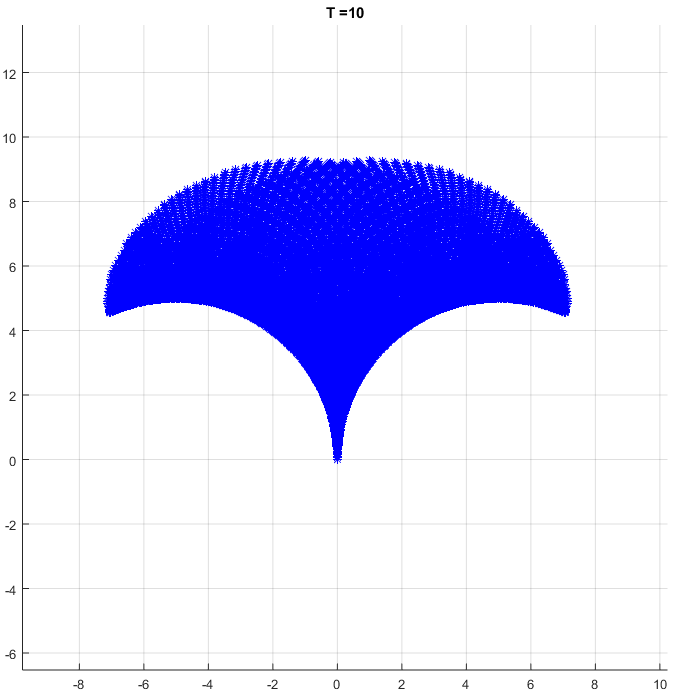
\includegraphics[width=5cm,height=5cm,keepaspectratio]{CC_2.png}}%[width=\textwidth]{a12_1.png}
%      			 \caption{A.}
%        		 \label{fig:cc_1}
      		 \end{subfigure}
      		 &
      		 \begin{subfigure}[b]{0.35\columnwidth}
			\parbox[c]{1em}{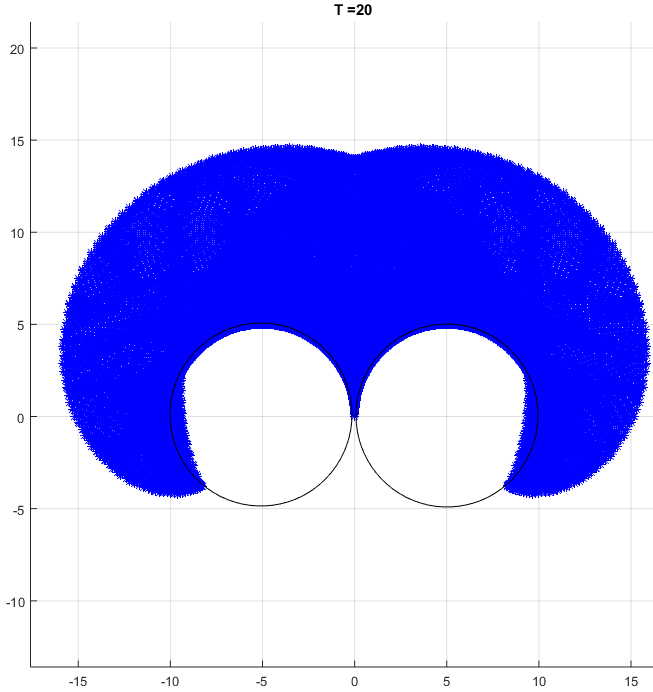
\includegraphics[width=5cm,height=5cm,keepaspectratio]{CC_4.png}}
%      			 \caption{A.}
%        		 \label{fig:cc_2}
      		 \end{subfigure}
      		 &
      		 \begin{subfigure}[b]{0.35\columnwidth}
			\parbox[c]{1em}{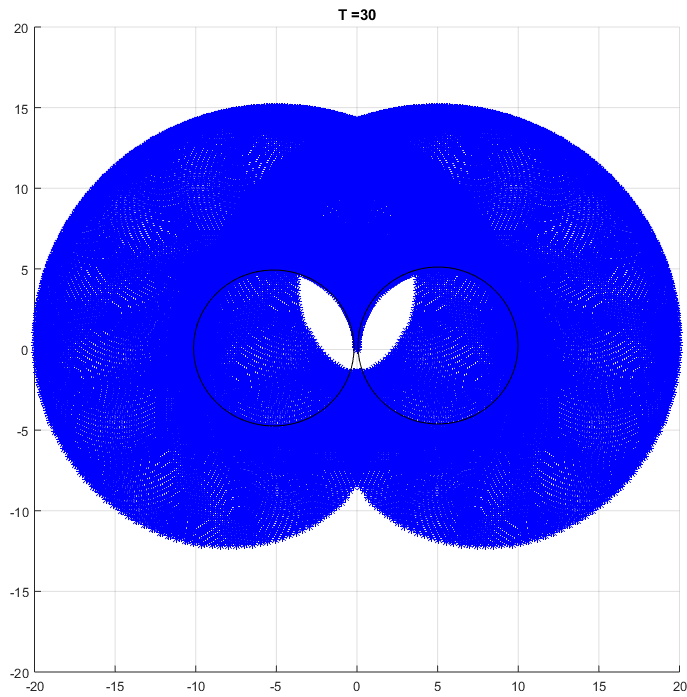
\includegraphics[width=5cm,height=5cm,keepaspectratio]{CC_5.png}}
%     			 \caption{A.}
%        		 \label{fig:CL_set}
      		 \end{subfigure}
      		 
	\end{tabular}
	\caption{Reachability set for CC trajectories}
	\label{fig:CC_set}
\end{figure}

\begin{figure}[H]
	\begin{tabular}{ccc}
		\begin{subfigure}[b]{0.35\columnwidth}
			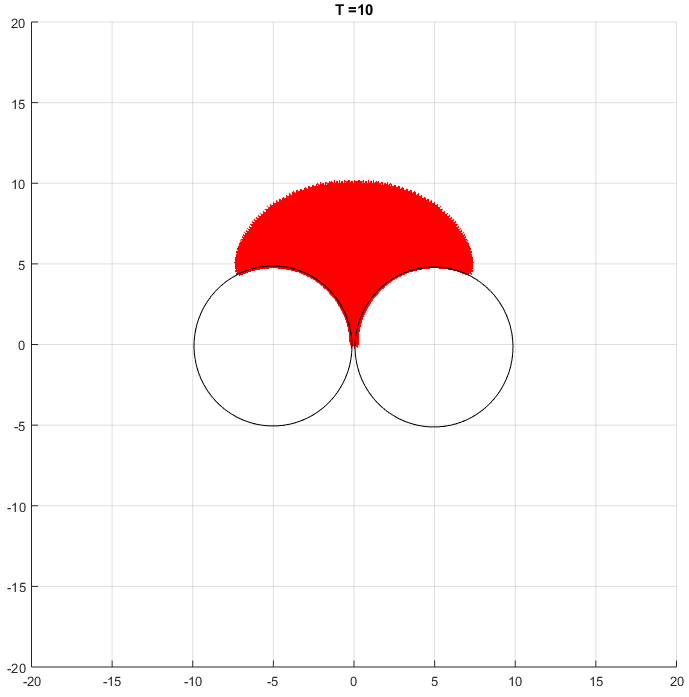
\includegraphics[width=5cm,height=5cm,keepaspectratio]{CL_1.png}%[width=\textwidth]{a12_1.png}
%      			 \caption{A.}
%        		 \label{fig:cc_1}
      		 \end{subfigure}
      		 &
      		 \begin{subfigure}[b]{0.35\columnwidth}
			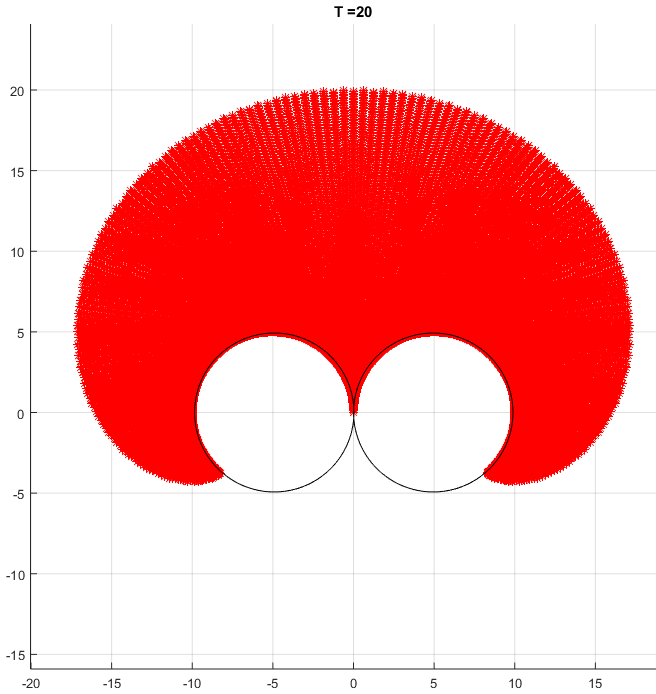
\includegraphics[width=5cm,height=5cm,keepaspectratio]{CL_2.png}
%      			 \caption{A.}
%        		 \label{fig:cc_2}
      		 \end{subfigure}
      		 &
      		 \begin{subfigure}[b]{0.35\columnwidth}
			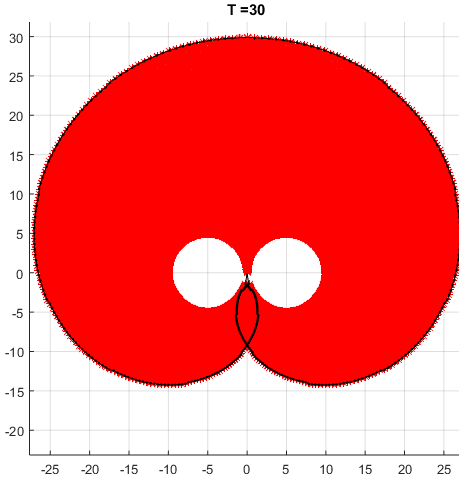
\includegraphics[width=5cm,height=5cm,keepaspectratio]{CL_3.png}
%      			 \caption{A.}
%        		 \label{fig:cc_3}
      		 \end{subfigure}
	\end{tabular}
	\caption{Reachability set for CS trajectories}
	\label{fig:CS_set}
\end{figure}

\subsection{Single agent case}
The car was initially programmed to reach the origin, starting from any initial position $(x_0,y_0,\theta_0)$, without constraints on angle of arrival. The initial position was taken such that its distance from origin is sufficiently larger than minimum radius of turning. In this case, according to \cite{cockayne}, the shortest path will be a CS trajectory. This can be described as a combination of an arc and a tangent to one of the circles of minimum radius. This is was implemented using the feedback strategy: \\
%put this in box
\begin{algorithm}[H]
\caption{Reach (0,0)}
\begin{algorithmic} 
\WHILE{$\sqrt{x^2 + y^2} \geq \epsilon$}
\IF{$\theta - \tan^{-1}(y/x) \leq \rho$}
\STATE $u = 0$
\ELSIF{$\theta - \tan^{-1}(y/x) \leq 0$}
\STATE $u = -u_{max}$
\ELSE
\STATE $u = u_{max}$
\ENDIF
\STATE update $\theta$, x and y
\ENDWHILE
\end{algorithmic}
\end{algorithm}
% include a pic of motion
But this feedback law fails in the situation when final position lie within $C_R$ or $C_L$. Thus to look at the nearby points we need to modify our solution.

\subsection{Characterization of 2-D plane}
The strategy for reaching any point in the 2-D plane can be described as follows. 
Any point outside$C_R$ and $C_L$ can be reached time optimally by a CS trajectory. Whereas, any point within them can be reached optimally by a CC trajectory.
This can be proven as follows:
%write proof
\begin{enumerate}[I]
\item Take a point outside the circles. CS and CC trajectory are common till point A. Beyond that the shortest path from A to P is a straight line.
\item Take a point inside $C_R$. Draw a circle of minimum radius passing through B and tangent to $C_L$. This intersects $C_L$ at P. Thus, CS and CC trajectory are common till point P (Figure 3). To prove that CC is optimal we need to show 
\begin{equation}
\begin{aligned}
R(2\pi - \phi) + l &\geq r(2\pi - \theta))\\
\textrm{or}\; l &\geq R(\phi - \theta) = R\alpha\\
\textrm{Since }\phi \geq \theta, \textrm{we have } l &\geq R\,tan\alpha\\
\textrm{As }\alpha \in [0, \pi/2], R\,tan\alpha &\geq  R\alpha
\end{aligned}
\end{equation}
\begin{figure}[H]
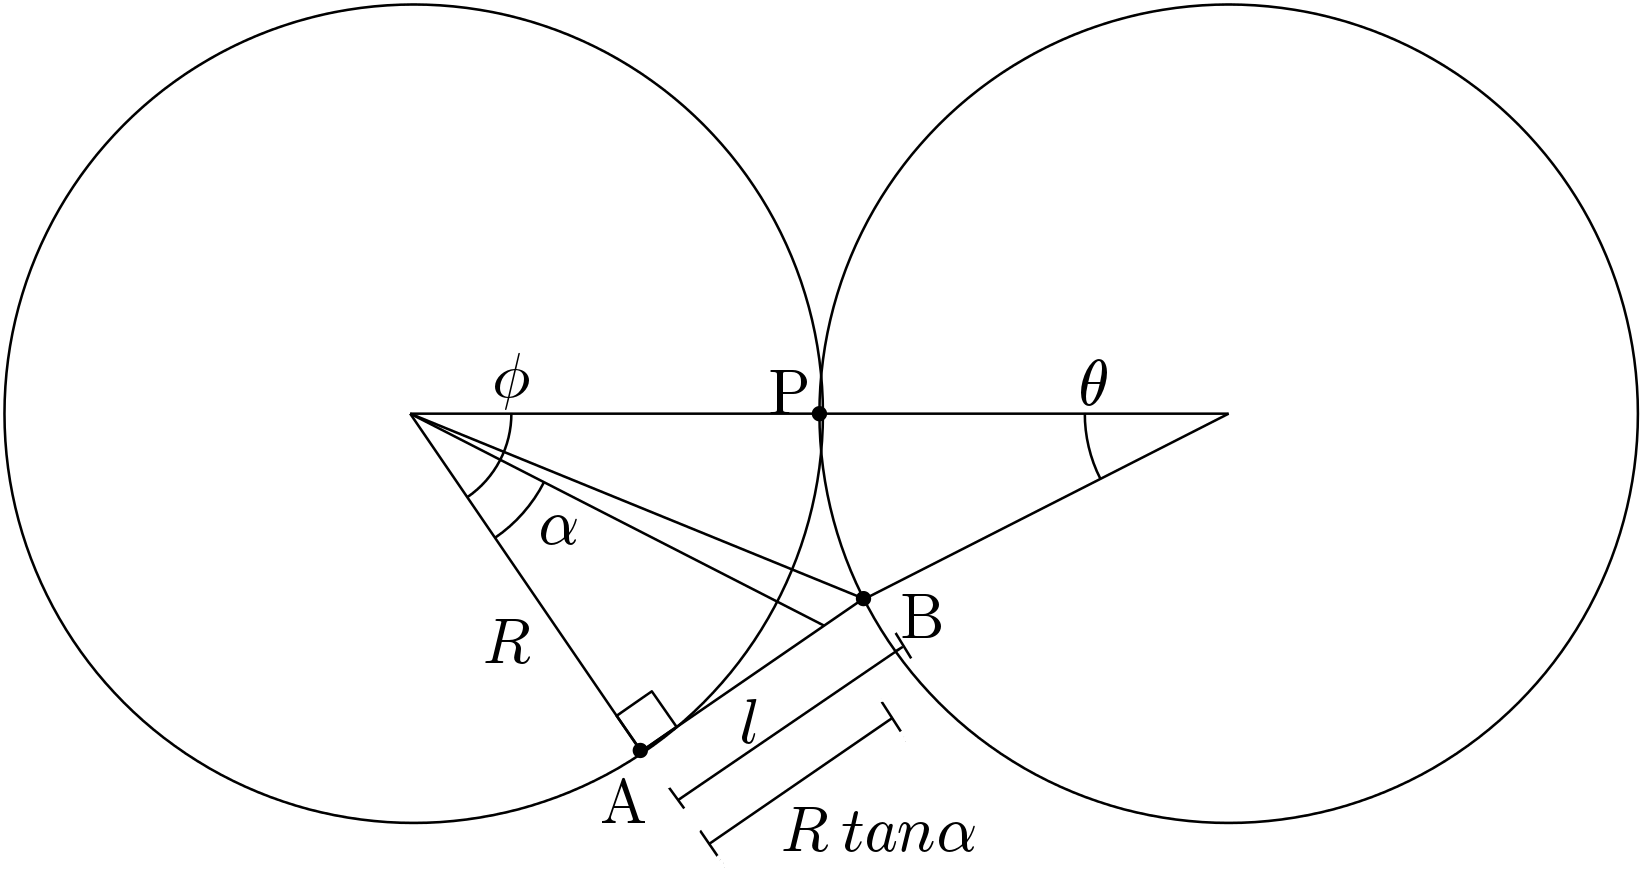
\includegraphics[width=10cm,height=10cm,keepaspectratio]{CC_proof.png}
\label{fig:cc_proof}
\caption{Proof of CC case}
\end{figure}

\end{enumerate} 
\section{Two vehicle case}
Following a similar approach as for one vehicle case, the rendezvous problem of two vehicles can be looked at by dividing the plane in different sections based on their initial positions and searching for time optimal trajectories of both the vehicles. Let $d$ be the distance between the two vehicles. A rectangular coordinate system is chosen such that its origin is at position of vehicle A, $P_A =  (0,0)$ and the positive direction of x-axis is towards vehicle B, $P_B = (d,0)$. Let $\alpha$ and $\beta$ be the angles their initial orientations make with the positive x-axis when measured counter-clockwise. 

\subsection{Equivalency Groups}
The classification of plane can be proceeded by first dividing the range of possible orientations $\alpha$ and $\beta$ in four quadrants. Quadrant 1 corresponds to the range $[0, \pi/2]$, quadrant 2 to $[\pi/2, \pi]$, quadrant 3 to $[\pi/3,\pi/2]$, and quadrant 4 to the range [3$\pi/$2, 2$\pi$]. Since $\alpha$ and $\beta$ can be in any of the four quadrants, there are 16 different possible combinations of quadrants. We represent those 16 by a $4\times4$ matrix, $\{a_{ij}\}$, where index $i$ corresponds to the quadrant number of vehicle A, and index $j$ of vehicle B.

Element $a_{ij}$ therefore describes the class of all paths whose initial and final orientation angles ($\alpha$, $\beta$) belong to the quadrants $i$ and $j$ , respectively. For example, the case $\alpha \in [0, \pi/2]$, $\beta \in [\pi/2, \pi]$ corresponds to the element $a_{12}$ and covers all those paths whose orientation angles belong to the first and second quadrant, respectively.

It will be shown below that these 16 classes can be reduced to six independent clusters, called equivalency groups. We consider two trajectories to be equivalent if one can be converted into another by taking a reflection along x or y axis.

$\textbf{Proposition:}$ Let $T_{\alpha,\beta}$ be the optimum trajectories for vehicle A and B together, then following trajectories are equivalent:

$T_{\alpha,\beta} \simeq T_{\pi-\beta,\pi-\alpha}$

$T_{\alpha,\beta} \simeq T_{-\alpha,-\beta} $.\\
This leads to following equivalency groups:
\begin{table}[H]
\centering
\begin{tabular}{ll}
$a_{11} \simeq a_{22}  \simeq a_{33} \simeq a_{44}$		& $a_{14} \simeq a_{23} \simeq a_{32} \simeq a_{41}$\\
$a_{12} \simeq a_{43}$ 		&  $a_{21} \simeq a_{34}$\\ 
$a_{13} \simeq a_{42}$ 		&  $a_{24} \simeq a_{31}$
\end{tabular}
\end{table}
Each of these six equivalent groups are discussed by varying the distance between the vehicles.\\
There are three possible scenarios for rendezvous. One is both vehicles move for the same duration till they meet at a point. Another is when one vehicle moves for a longer duration than another vehicle. We call this trajectory to be degenerate in second vehicle.
Last possibility is for one vehicle to reach the initial position of the other directly. The first two cases are denoted by T[CS CS] and third one is denoted by T[CS 0] or T[0 CS].

\subsection{$a_{11}$}
Let $d_1$ be the minimum distance at which direct path to initial position of B by vehicle A is optimal. Similarly let $d_2$ be the minimum distance at which T[LS LS] is the optimal trajectory and  $d_3$ be the minimum distance at which T[RS LS] is the optimal trajectory. \\
%\textbf{Claim:} $d_1 \leq d_2$ and $d_1 \leq d_2$ for all values of $\alpha$ and $\beta$ in $a_{11}$.\\
If the distance between the two vehicles, d, is less than $d_1$ then the path followed by A and B is RS and LS respectively.\\
Now if $d_2$ is less than $d_3$, following sequence of optimal trajectories is followed:
\begin{itemize}
\item T[RS 0] for $d_1 \leq d \leq d_2$
\item T[LS LS] for $d_2 \leq d \leq d_3$
\item T[RS LS]  for $d_3 \leq d \leq d_4$
\end{itemize}
Else if $d_3 \geq d_4$, then sequence is:
\begin{itemize}
\item T[RS 0] for $d_1 \leq d \leq d_3$
\item T[RS LS]  for $d_3 \leq d \leq d_4$
\end{itemize}
\begin{figure}[H]
	\begin{tabular}{cc}
		\begin{subfigure}[b]{0.4\columnwidth}
			\parbox[c]{1em}{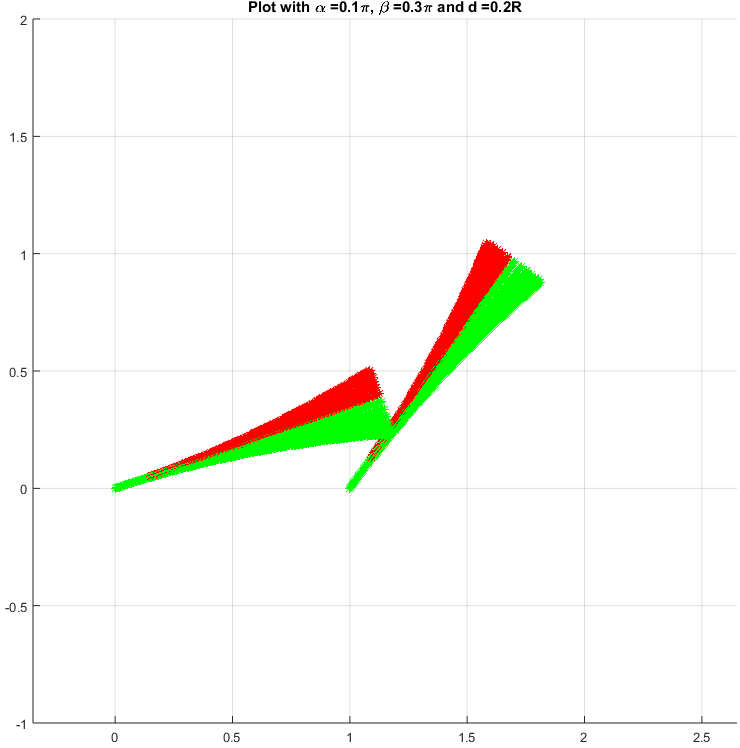
\includegraphics[width=6cm,height=6cm,keepaspectratio]{a11_2.png}}%[width=\textwidth]{a12_1.png}
%      			 \caption{A.}
        		 \label{fig:a13_1}
      		 \end{subfigure}
      		 &
      		 \begin{subfigure}[b]{0.4\columnwidth}
			\parbox[c]{1em}{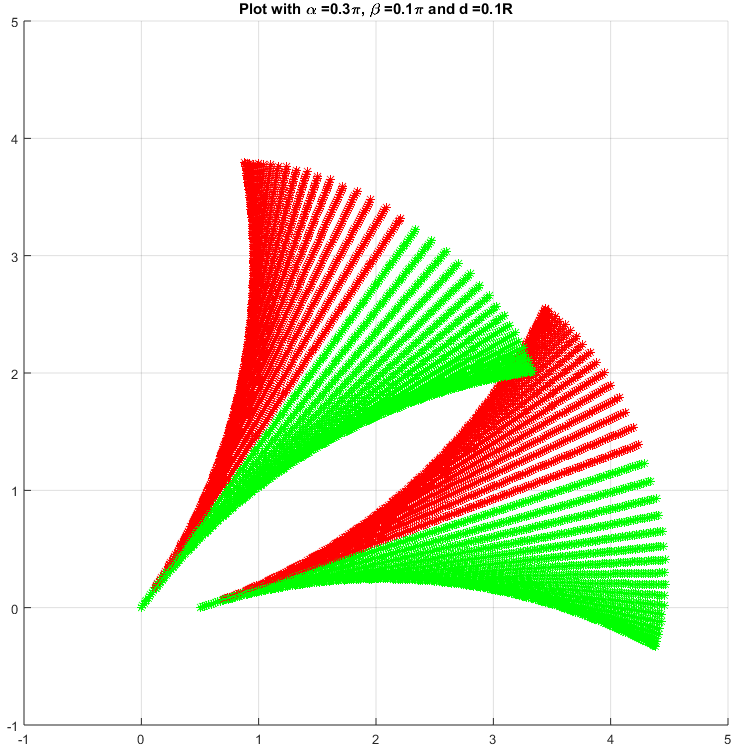
\includegraphics[width=6cm,height=6cm,keepaspectratio]{a11.png}}
%      			 \caption{A.}
        		 \label{fig:a13_2}
      		 \end{subfigure}
      		 \\
      		 \begin{subfigure}[b]{0.4\columnwidth}
			\parbox[c]{1em}{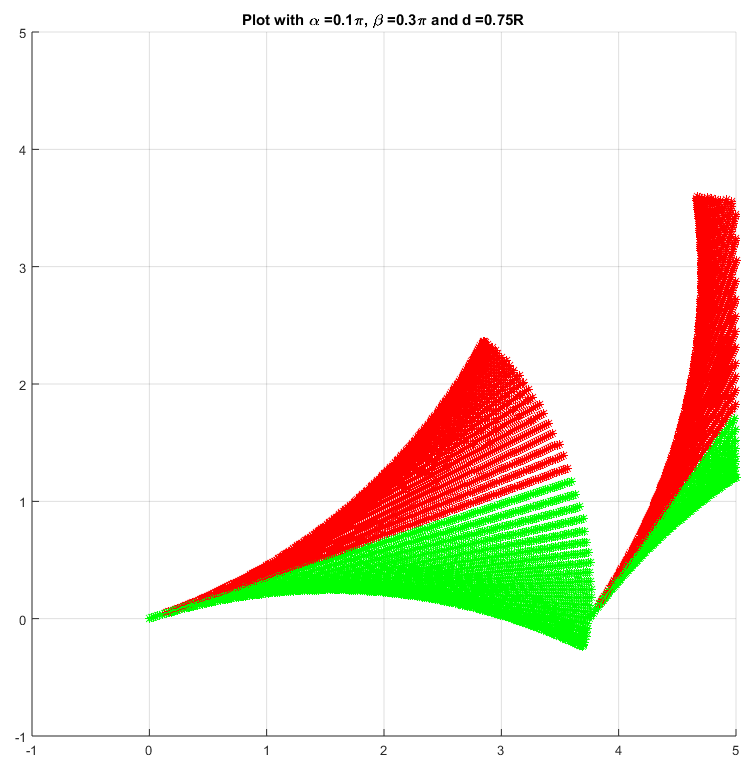
\includegraphics[width=6cm,height=6cm,keepaspectratio]{a11_3.png}}
%      			 \caption{A.}
        		 \label{fig:a13_3}
      		 \end{subfigure}
      		  &
      		 \begin{subfigure}[b]{0.4\columnwidth}
			\parbox[c]{1em}{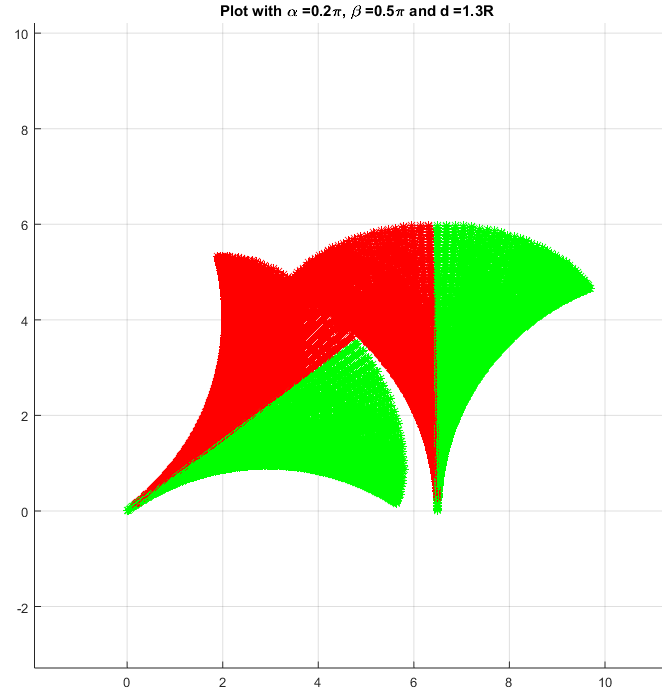
\includegraphics[width=6cm,height=6cm,keepaspectratio]{a11_5.png}}
%      			 \caption{A.}
        		 \label{fig:a13_4}
      		 \end{subfigure}
	
	\end{tabular}
	\caption{Trajectories for $a_{11}$}
\end{figure}
%The path can be degenerate in B only, thus the reaching time is decided by path of A.
For all values of d, T[RS,LS] $\leq$ T[RS,RS] as any point on the right of line passing through B and at angle $\beta$ is reached by A later than the corresponding point on the line.
Similarly we can prove T[RS,LS] $\leq$ T[LS,RS]. 

\subsection{$a_{12}$}
Let $d_1$ be the distance at which straight line path by one vehicle and CS by other is optimal. Then we can write the sequence of optimal trajectories as:
\begin{itemize}
\item For $0 < d \leq d_1$
\begin{itemize}
\item For $\alpha \leq \pi-\beta$ T[LS LS]
\item For $\alpha \geq \pi-\beta$ T[RS RS]
\end{itemize}
\item For $d_1 \leq d$ T[RS LS]
\end{itemize}
\begin{figure}[H]
	\begin{tabular}{@{\extracolsep{\fill}}l @{\extracolsep{\fill}}l @{\extracolsep{\fill}}l}
		\begin{subfigure}[b]{0.35\columnwidth}
			\parbox[c]{1em}{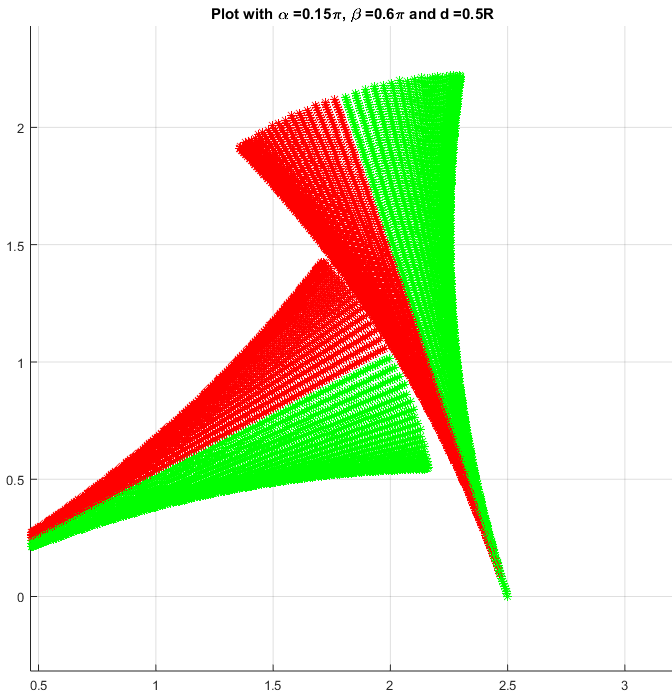
\includegraphics[width=5cm,height=5cm,keepaspectratio]{a12_2.png}}%[width=\textwidth]{a12_1.png}
%      			 \caption{A.}
        		 \label{fig:a12_1}
      		 \end{subfigure}
      		 &
      		 \begin{subfigure}[b]{0.35\columnwidth}
			\parbox[c]{1em}{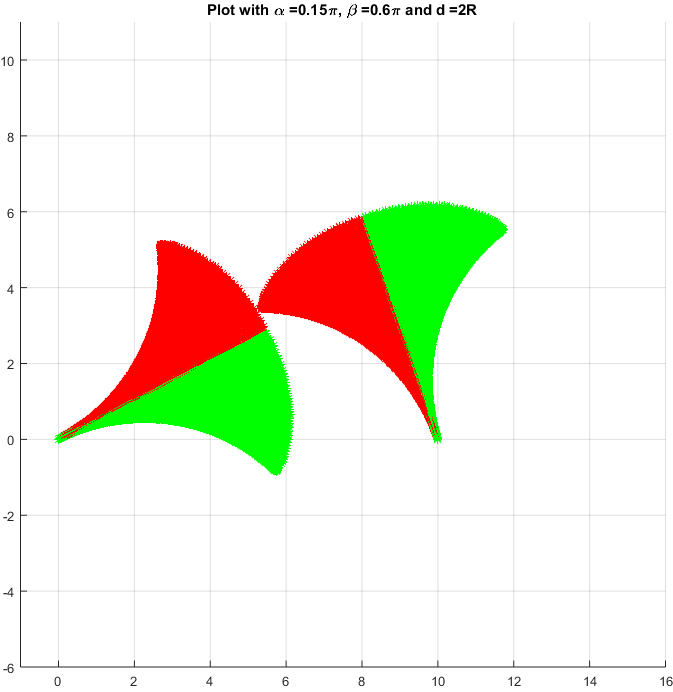
\includegraphics[width=5cm,height=5cm,keepaspectratio]{a12_3.png}}
%      			 \caption{A.}
        		 \label{fig:a12_2}
      		 \end{subfigure}
      		 &
      		 \begin{subfigure}[b]{0.35\columnwidth}
			\parbox[c]{1em}{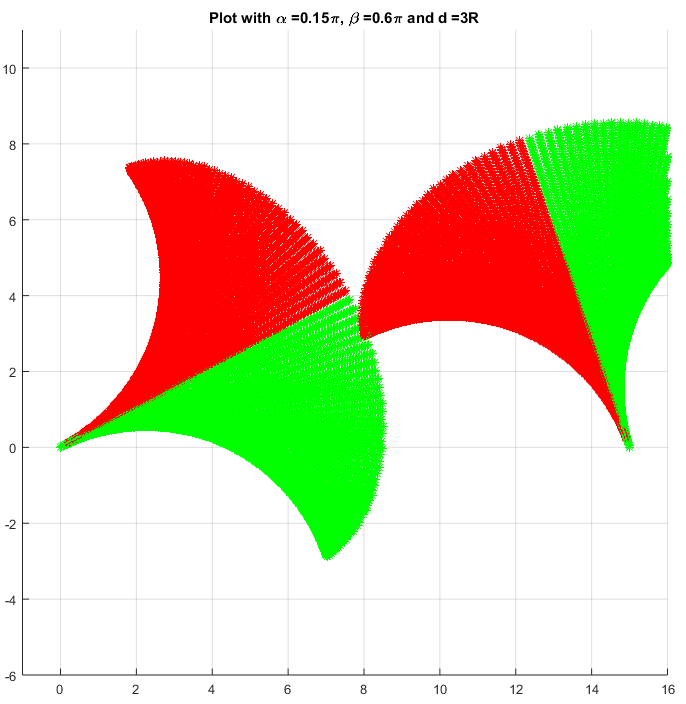
\includegraphics[width=5cm,height=5cm,keepaspectratio]{a12_1.png}}
%      			 \caption{A.}
        		 \label{fig:a12_3}
      		 \end{subfigure}
	\end{tabular}
	\caption{A12}
\end{figure}

 
\subsection{$a_{13}$}
\begin{itemize}
\item If both are inside each other's circles of minimum radius:
\begin{itemize}
\item For $\alpha \leq -\pi+\beta$ T[LS RS]
\item For $\alpha \geq -\pi+\beta$ T[RS LS]
\end{itemize}
\item If both are outside each other's circles:
\begin{itemize}
\item T[RS RS]
\end{itemize}
\item If one is inside and other is outside:
\begin{itemize}
\item For B inside A's circle: T[RS RS] or T[0 RS]
\item For A inside B's circle: T[LS L] or T[LS 0]
\end{itemize}
\end{itemize}

\begin{figure}[H]
	\begin{tabular}{cc}
		\begin{subfigure}[b]{0.4\columnwidth}
			\parbox[c]{1em}{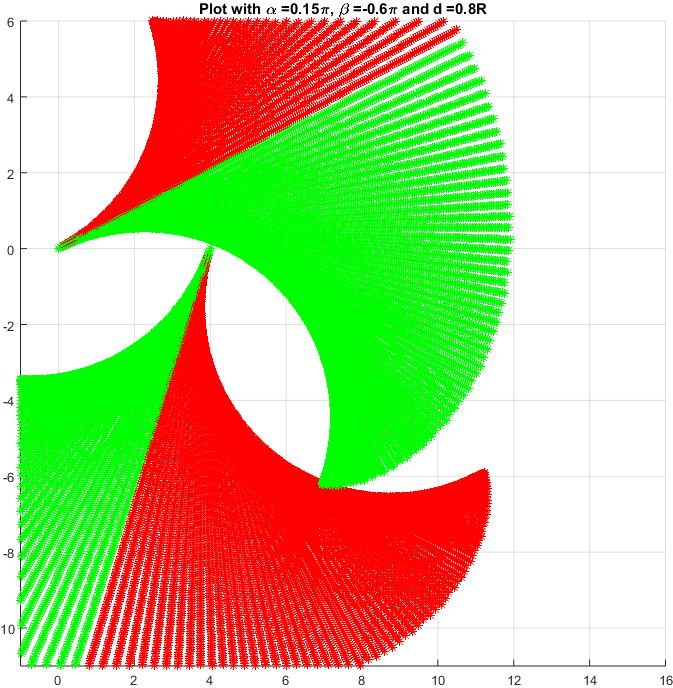
\includegraphics[width=6cm,height=6cm,keepaspectratio]{a13_1.png}}%[width=\textwidth]{a12_1.png}
%      			 \caption{A.}
        		 \label{fig:a13_1}
      		 \end{subfigure}
      		 &
      		 \begin{subfigure}[b]{0.4\columnwidth}
			\parbox[c]{1em}{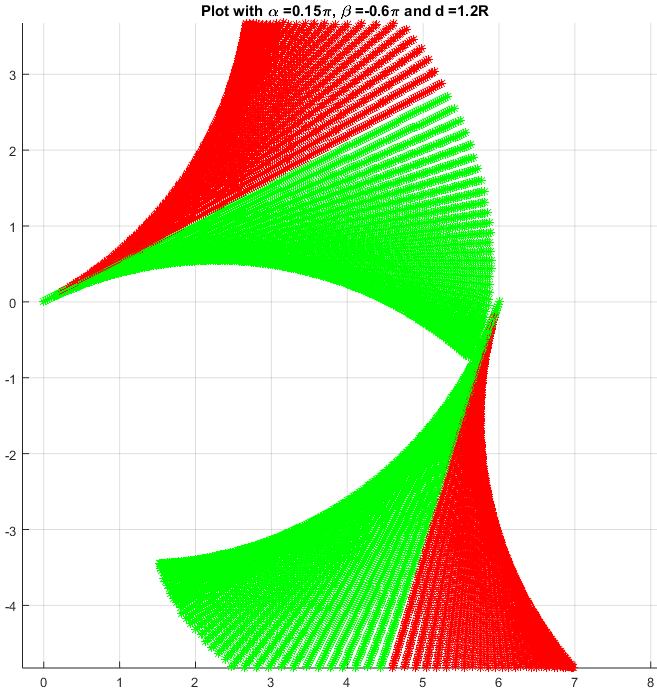
\includegraphics[width=6cm,height=6cm,keepaspectratio]{a13_2.png}}
%      			 \caption{A.}
        		 \label{fig:a13_2}
      		 \end{subfigure}
      		 \\
      		 \begin{subfigure}[b]{0.4\columnwidth}
			\parbox[c]{1em}{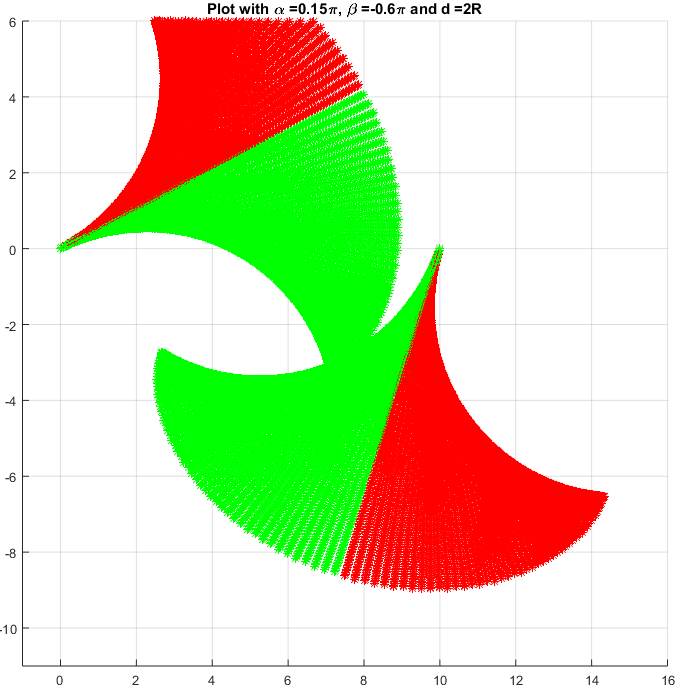
\includegraphics[width=6cm,height=6cm,keepaspectratio]{a13_3.png}}
%      			 \caption{A.}
        		 \label{fig:a13_3}
      		 \end{subfigure}
      		  &
      		 \begin{subfigure}[b]{0.4\columnwidth}
			\parbox[c]{1em}{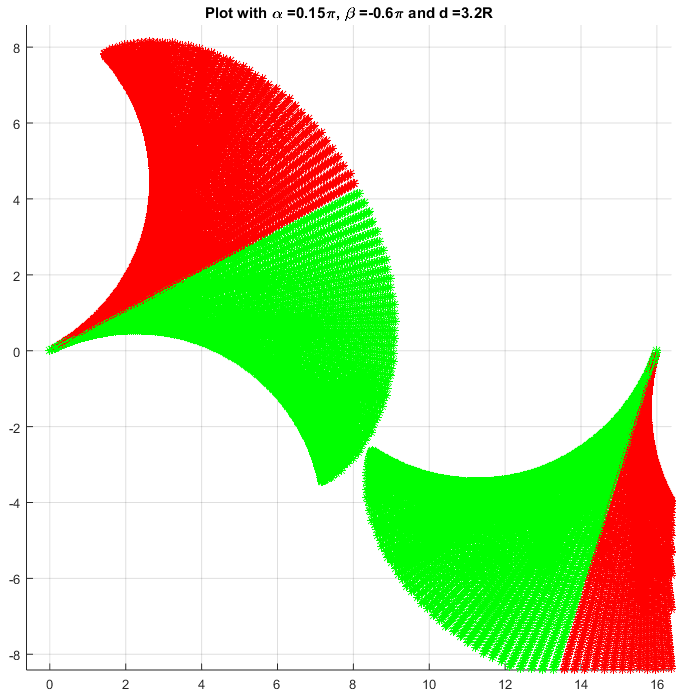
\includegraphics[width=6cm,height=6cm,keepaspectratio]{a13_4.png}}
%      			 \caption{A.}
        		 \label{fig:a13_4}
      		 \end{subfigure}
	\end{tabular}
	\caption{A13}
\end{figure}

\subsection{$a_{14}$}
\begin{itemize}
\item If B lies in the circle of A:
\begin{itemize}
\item T[RS L]
\end{itemize}
\item If B lies outside the circle of A, in increasing order of distance:
\begin{itemize}
\item T[RS 0]
\item T[RS R]
\item T[RS RS]
\end{itemize}
\end{itemize}
\begin{figure}[H]
	\begin{tabular}{@{\extracolsep{\fill}}l @{\extracolsep{\fill}}l @{\extracolsep{\fill}}l}
		\begin{subfigure}[b]{0.35\columnwidth}
			\parbox[c]{1em}{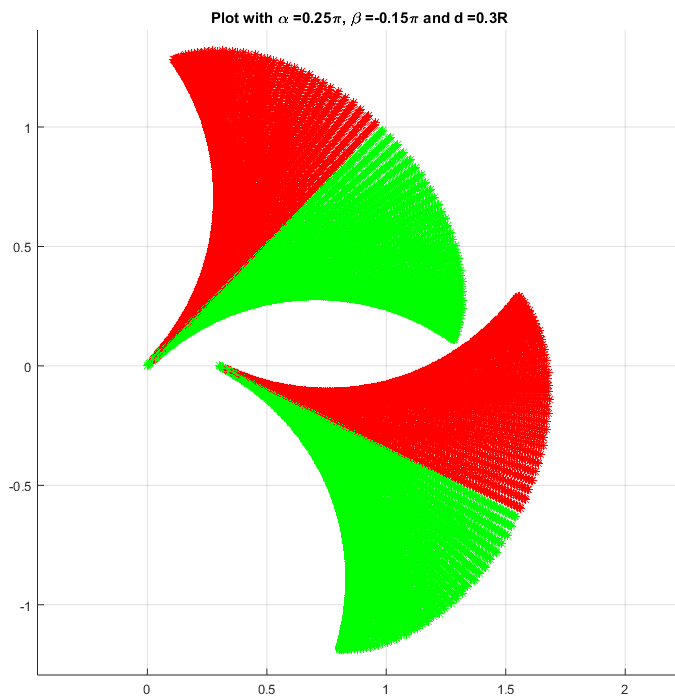
\includegraphics[width=5cm,height=5cm,keepaspectratio]{a14_1.png}}%[width=\textwidth]{a12_1.png}
%      			 \caption{A.}
        		 \label{fig:a12_1}
      		 \end{subfigure}
      		 &
      		 \begin{subfigure}[b]{0.35\columnwidth}
			\parbox[c]{1em}{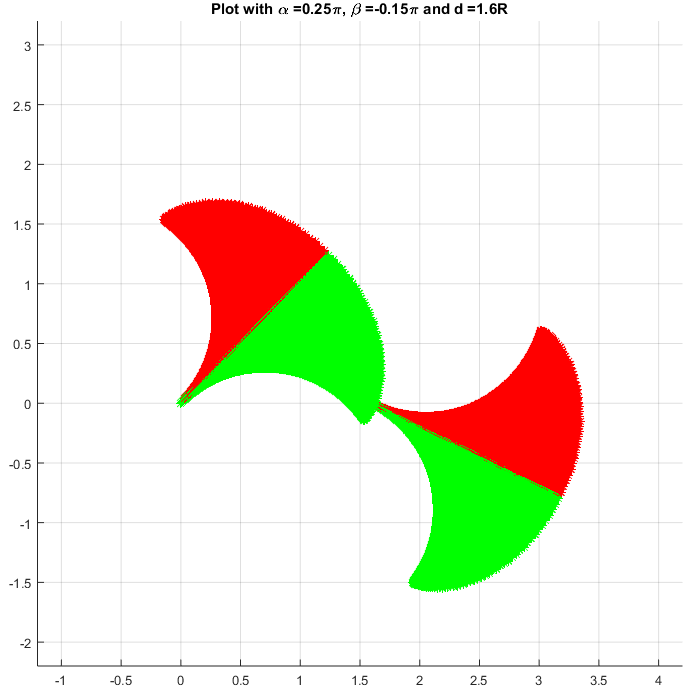
\includegraphics[width=5cm,height=5cm,keepaspectratio]{a14_2.png}}
%      			 \caption{A.}
        		 \label{fig:a12_2}
      		 \end{subfigure}
      		 &
      		 \begin{subfigure}[b]{0.35\columnwidth}
			\parbox[c]{1em}{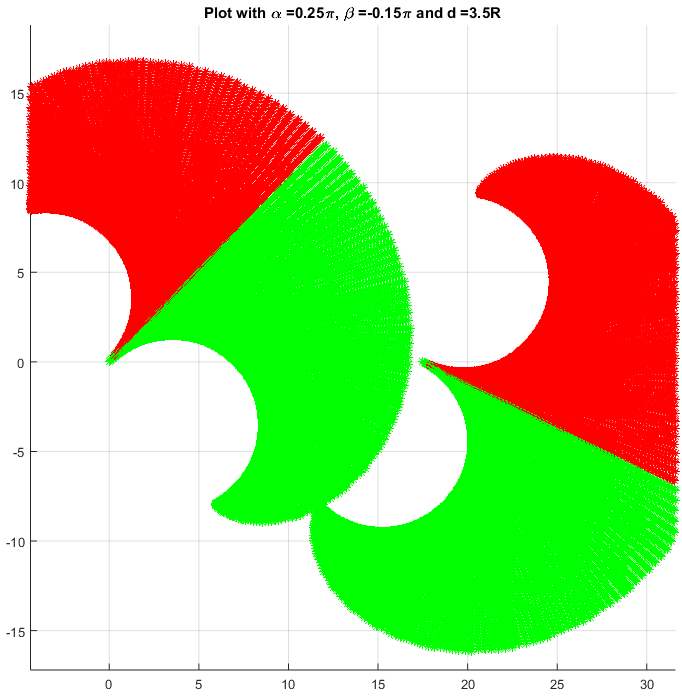
\includegraphics[width=5cm,height=5cm,keepaspectratio]{a14_3.png}}
%      			 \caption{A.}
        		 \label{fig:a12_3}
      		 \end{subfigure}
	\end{tabular}
	\caption{A14}
\end{figure}

\subsection{$a_{21}$}
The optimal trajectory is T[RS LS] for all distances.\\
This can be proved as any CS curve starting from A will intersect the straight line passing through B ($S_B$) at angle $\beta$ before any point on the right of $S_B$. Thus T[RS LS] $\leq$ T[RS RS]. Similarly T[RS LS] $\leq$ T[LS RS] and T[RS LS] $\leq$ T[LS RS].
\begin{figure}[H]
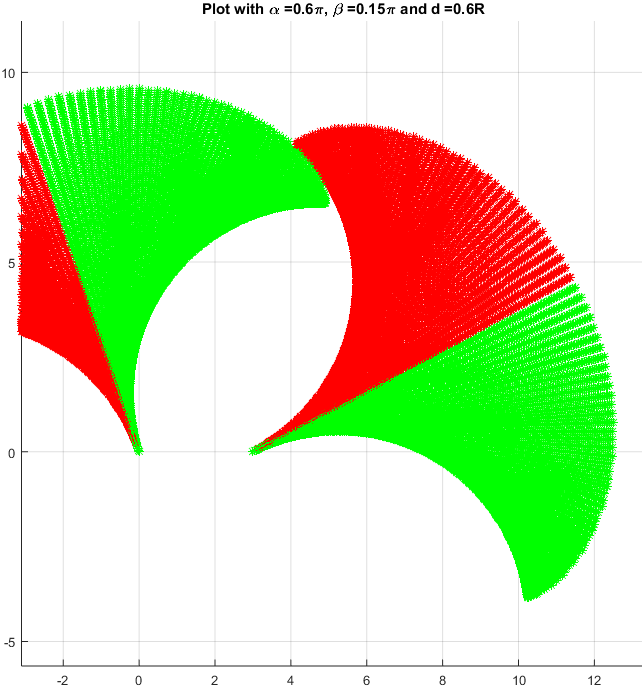
\includegraphics[width=6cm,height=6cm,keepaspectratio]{a21_1.png}
\caption{A21}
\end{figure}
\subsection{$a_{24}$}
For $\pi-\alpha \leq 2\pi-\beta$ T[LS RS]\\
For $\pi-\alpha \geq 2\pi-\beta$ T[RS LS]

\section{Curvature}
Meeting of two vehicles can be seen as the intersection of their rechability sets. Radius of curvature of the reachability set can be used to find intersection them.\\
Radius of curvature decreases uniformly as turning time increases from 0 to T. It reduces to 0 at t = T, implying that is a corner point. 

\section{Types of paths}
The meeting of two vehicles can occur by one of the four possible paths:
\begin{itemize}
\item Along the common tangent
\item At the intersection of two circles of minimum radius 
\item At the initial position of one of the vehicles : direct
\item At a point on minimum radius circle of one, reached by a CS path by another, with nonzero S: CSC
\end{itemize}

$\textbf{Proposition:}$ Time optimal point of intersection for two vehicles cannot lie within any of the four circles of minimum radius. In other words trajectotry for anyone of them cannot be CC.

$\textbf{Proposition:}$ Intersection of CS paths by both vehicles is along common tangent.

Proof: For a time optimal meeting, intersection of paths occurs as the the boundaries of reachability set of both vehicles. Let the boundary made by CS paths be called outer boundary and that made by C alone be called inner boundary. Thus intersection of CS paths by both vehicles happens on intersection of outer boundaries of both at one point. 

The above four paths can be seen from these two propositions. Since CC is ruled out, we have four possible trajectories for each vehicle: CS (with both C and L of non-zero length), C, S and zero (both C and S are zero). This gives following cases:

\begin{table}[H]
\centering
\begin{tabular}{|c|c|c|c|c|}
\hline
\textbf{} & \textbf{CS} & \textbf{C} & \textbf{S} & \textbf{zero} \\ \hline
\textbf{CS} & common tangent & CSC & common tangent & direct \\ \hline
\textbf{C} & CSC & circle intersection & CSC & direct \\ \hline
\textbf{S} & common tangent & CSC & common tangent & direct \\ \hline
\textbf{zero} & direct & direct & direct & - \\ \hline
\end{tabular}
\end{table}

\begin{itemize}
\item[--] If both the vehicles are in each other's circles of minimum radius, only intersection of circles and CSC are possible
\item[--] If the distance between vehicles is greater that 4R the intersection is always along common tangent
\item[--] $a_{12}$ and $a_{21}$ do not have a direct path for any value of d
\end{itemize}

\section{Rendezvous point calculation}
 Optimal path can be determined by calculating the path length for the four possible cases given in above section and choosing the minimum time taking one. For the case of common tangent, total path length along circles and tangent need to be calculated and divided in two to give time of one vehicle.  For the case of intersection of circles is intersection point is computed and length along the arc for both is calculated separately. Maximum of the two is used for calculating final time. Length along direct path can be calculated by treating as a single vehicle programmed to reach a predetermined point. 
 
 CSC requires a minimization routine. Here the outer boundary intersects with a point on inner boundary or at corner point. Since the outer boundary is always the time limiting path, we focus on the CS path only. Thus we need to minimize the time taken by CS path to intersect a point on the arc of the circle reached by other vehicle in lesser time.
  

\section{Future Work}
The observed sequences for each of the six cases remains to be proved. Next step would be to calculate the exact rendezvous point from knowledge of the initial state alone. Building on these, then further feedback based laws for the two vehicle case can be stated. We would further investigate the ways to generalize these results and methods for more than two vehicles.

\bibliography{ref}
\bibliographystyle{ieeetr}



\end{document}